\section{Event selections} \label{sec:event_selection}

For all three final states, the aim is to define a phase space in which di-Higgs signal sensitivity is maximized. 

In order to improve the signal extraction, methods involving DNNs were utilized for the
FH and SL channels. For the FL channel, a cut based analysis is performed as an MVA approach was deemed unfeasible 
due to low statistics in this channel. 

After event categorization is performed, a combined fit of the simulated \mgg distribution templates to data is performed simultaneously in all categories.

The number of leptons per event is used to ensure that an event cannot fall into multiple analysis categories. 
In order to pass the FH, SL, or FL selections, events are required to contain exactly zero, exactly one, or exactly two leptons, respectively. 
Additionally, all channels are required to contain at least one diphoton candidate based on the photon selections described in Sec. \ref{sec:Objects}.  

\subsection{Fully-hadronic category}

Events fall into the FH analysis category if they contain exactly zero leptons, and at least four AK4 jets. Additionally,
the leading (sub-leading) photon \pt associated with the diphoton candidate is required to have a ratio to the diphoton candidate's 
invariant mass of at least 1/3 (1/4). In this final state, a selection is not made on b-tagging score as a preselection, in order to use this as an 
input feature to the DNN in order to allow it to learn how best to use this score for event discrimination.

The Fully-Hadronic $HH\rightarrow WW\gamma\gamma$ channel phase-space has a large overlap with the $HH\rightarrow bb\gamma\gamma$,
and Fully-Hadronic $HH\rightarrow ZZ\gamma\gamma$ processes. Due to the difficulty in differentiating these similar di-Higgs final states, the contributions coming from these two additional channels
are treated as signal. This analysis is optimized for the $WW\gamma\gamma$ final state, in which hadronic W decays including b-jets are very rare. Therefore, events with b-jet candidates should be removed.
For this, a binary DNN was setup, acting as a ``$bb\gamma\gamma$ killer".
This helps remove the large contamination from the $bb\gamma\gamma$ and Fully-Hadronic $ZZ\gamma\gamma$ processes.
For the $bb\gamma\gamma$ killer DNN, a $bb\gamma\gamma$ sample was used as a signal. The list
of backgrounds used for the training includes Fully-Hadronic $WW\gamma\gamma$, diphoton, $\gamma+$jets, QCD, $tt\gamma\gamma$, and $tt\gamma$.

The modelling of QCD and $\gamma+$jets has a large underprediction in MC. This comes from the lower region of minimum photon ID MVA, defined as the minimum value of the photon MVA scores 
between the two photon candidates from the highest $\pt$ diphoton candidate in the event. In order to properly model these processes,
their shapes are defined using a data-driven technique using the data sideband, defined as the regions 100-115 and 135-180 GeV in the $m_{\gamma\gamma}$ spectrum, 
where a QCD and $\gamma+$jets dominant region in data, the low photon ID side-band (ID $<$ -0.7), is used to model these processes. 
This is performed in a similar way as described in \cite{Sirunyan:2020sum}.
The overall normalization of events from the low photon ID
side-band region should not be expected, a priori, to be the same as the number of QCD and $\gamma$+jets events in the pre-selection.
To address this, a simultaneous fit in the minimum and maximum photon ID MVA's, defined as the lower and greater photon ID values between the two photons making up the 
highest $\pt$ diphoton candidate in each event, is performed. This includes a simultaneous fit to data in the high-ID region (ID$>$-0.7) in the data sidebands, with the addition of 
$\gamma\gamma+$jets and tt from MC, to extract the QCD $+$ $\gamma+$jets normalization.

Additionally, a fully-connected binary DNN is trained in order to separate Fully-Hadronic WW$\gamma\gamma$ events from all other background events.
For this the list of backgrounds includes diphoton, $\gamma+$jets, QCD, $tt\gamma\gamma$ and $tt\gamma$.
Apart from the signal and background lists, the network architecture and input variables are the same as for the bb$\gamma\gamma$ killer DNN. The input features 
used for training of both DNN's are shown in Fig. \ref{fig:DNNinputvars}. Note that the FH DNNs make the use of additional jet information not available in the SL final state, described in Sec. \ref{sec:SL_Event_Selection}. 

The most important variables for the bb$\gamma\gamma$ killer, according to their Shapley ranking \cite{shapley_values}, are
the sum of b-tagging scores of the two jets with the highest b-tagging scores, $\Delta R (\gamma\gamma) (=\sqrt{\Delta \phi^2 + \Delta \eta^2})$,
leading jet b-tagging score, ratio of leading photon $\pt$ to the diphoton mass, leading jet $\pt$,  vector sum of $\pt$ of the leading four jets,
b-tagging score of sub-leading jet, invariant mass of the system of the four leading $\pt$ jets, and minimum $\Delta R$ separation between
diphoton candidate and the four leading jets.

The most important variables for signal extraction, according to their Shapley ranking, are $\Delta R (\gamma\gamma)$, 
ratio of the leading and sub-leading photon $\pt$'s to the diphoton mass,
leading 2 jet invariant mass, leading 4 jet invariant mass, minimum $\Delta R$ separation between
the diphoton candidate and the four leading jets, and the sum of b-tagging scores among the two jets with the highest
b-tagging scores. Fig.~\ref{fig:FH_DataMC_1} shows the control plot of the DNN output score and a leading importance variable. 

After computing the DNN output score for each event, events are placed into categories based on DNN score in order to maximize the sensitivity of the DNN categorization. 
To optimize the expected sensitivity, the expected ratio of signal yield to the square root of background yield in the signal region is computed using MC while varying the number of categories and bins. 
Additionally, a signal region definition of 122 to 128 GeV is used as this is the experimental resolution: A range centered aroudn the expected Higgs mass with a width roughly 1-2 times 
the expected signal width. Four categories are defined, with the corresponding DNN score boundaries: [0.1, 0.893, 0.969, 0.983, 1.0].

In this analysis, events with an HH$\rightarrow$WW$\gamma\gamma$ identifier DNN score less than 0.1 
are removed, and therefore are not used in categorization, nor in any analytic fitting. This is done because this region contains a large portion of background, and a very low portion of signal, and therefore has a negligible impact on the sensitivity of the analysis. Additionally,
this region is not used as a control region to reduce the uncertainty of MC in the signal region.

% Note that as the DNN output score is used to categorize events but is not used as a shape in the extraction of any results, any disagreements 
% between data and simulation could lead to a sub-optimal network, but would not lead to any bias in the 
% final results. 

\begin{figure}[!htbp]
  \centering 
  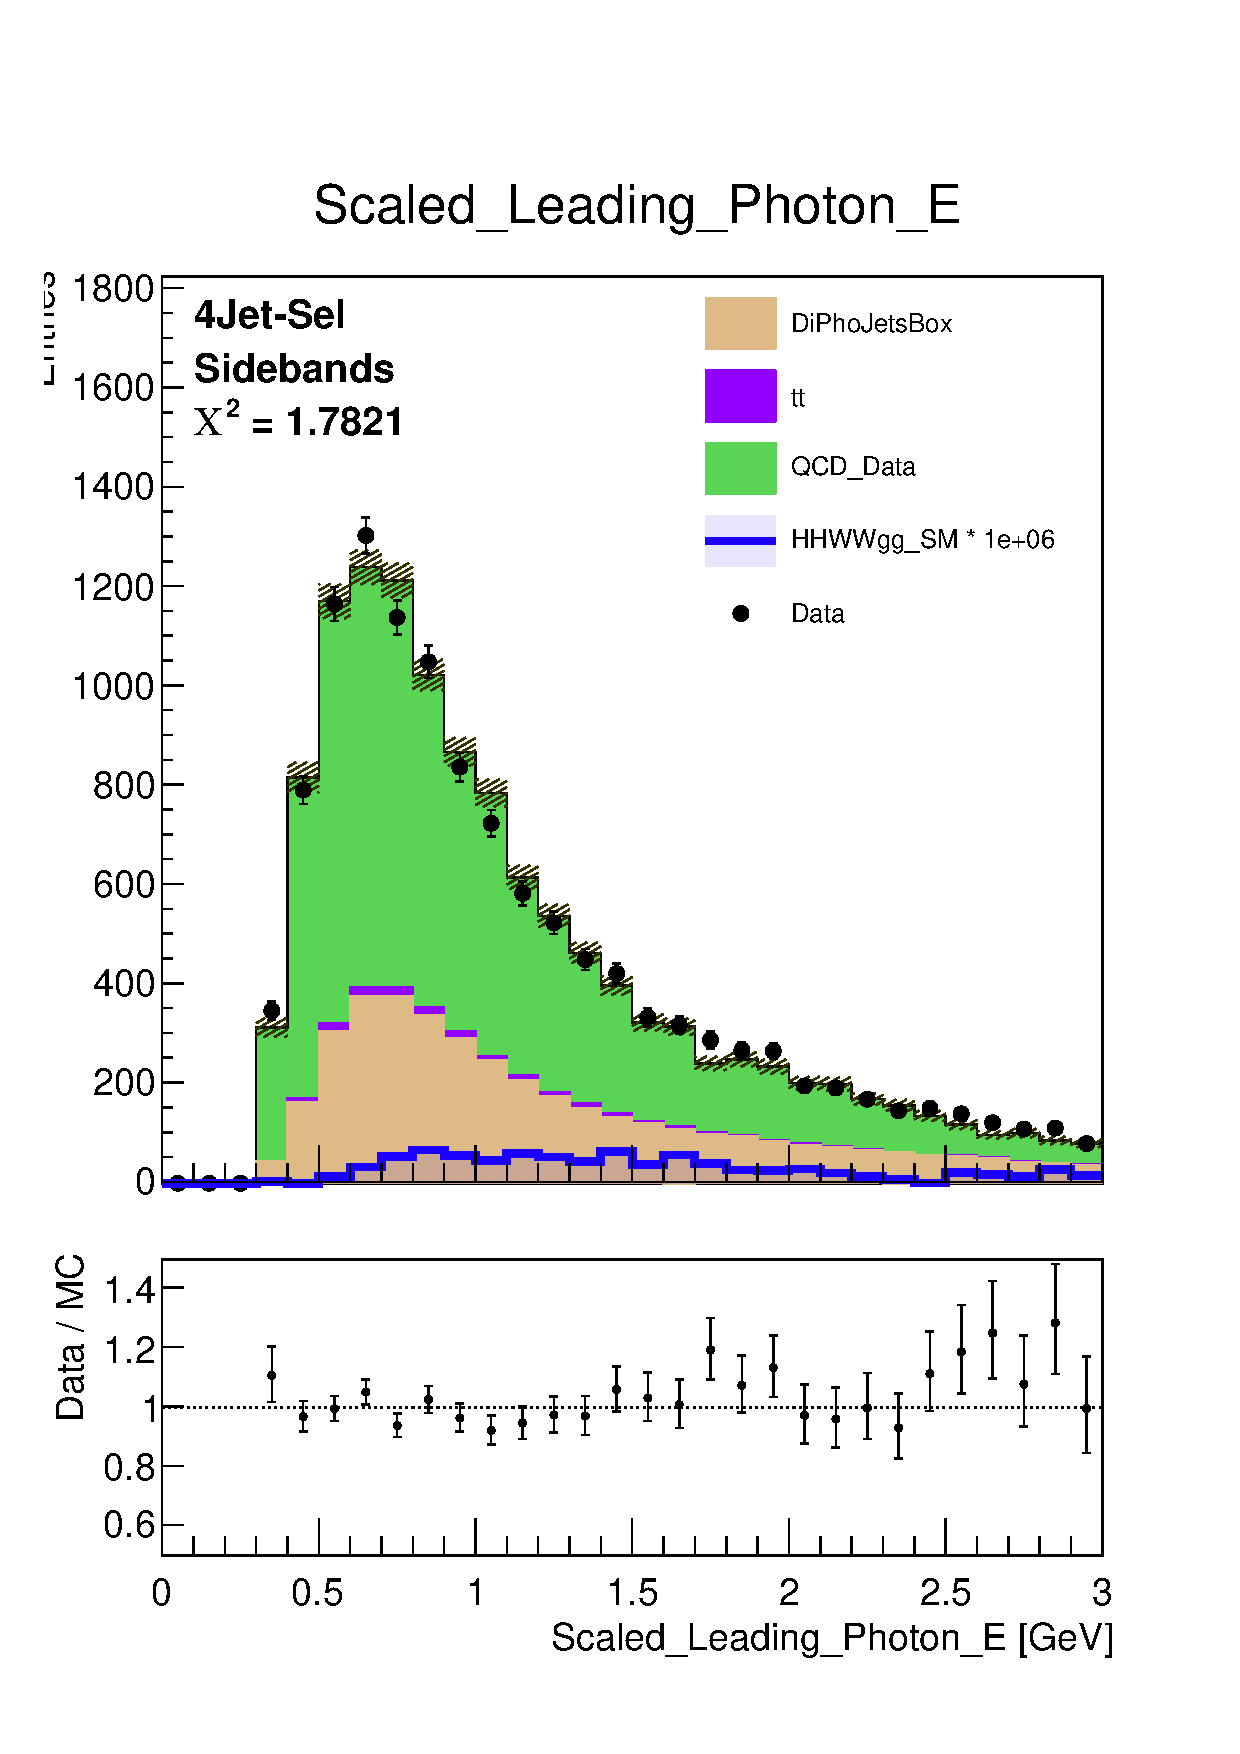
\includegraphics[width=0.45\textwidth]{Images/DataMC/DataMC_Scaled_Leading_Photon_E_SB_nonLog.pdf}%
  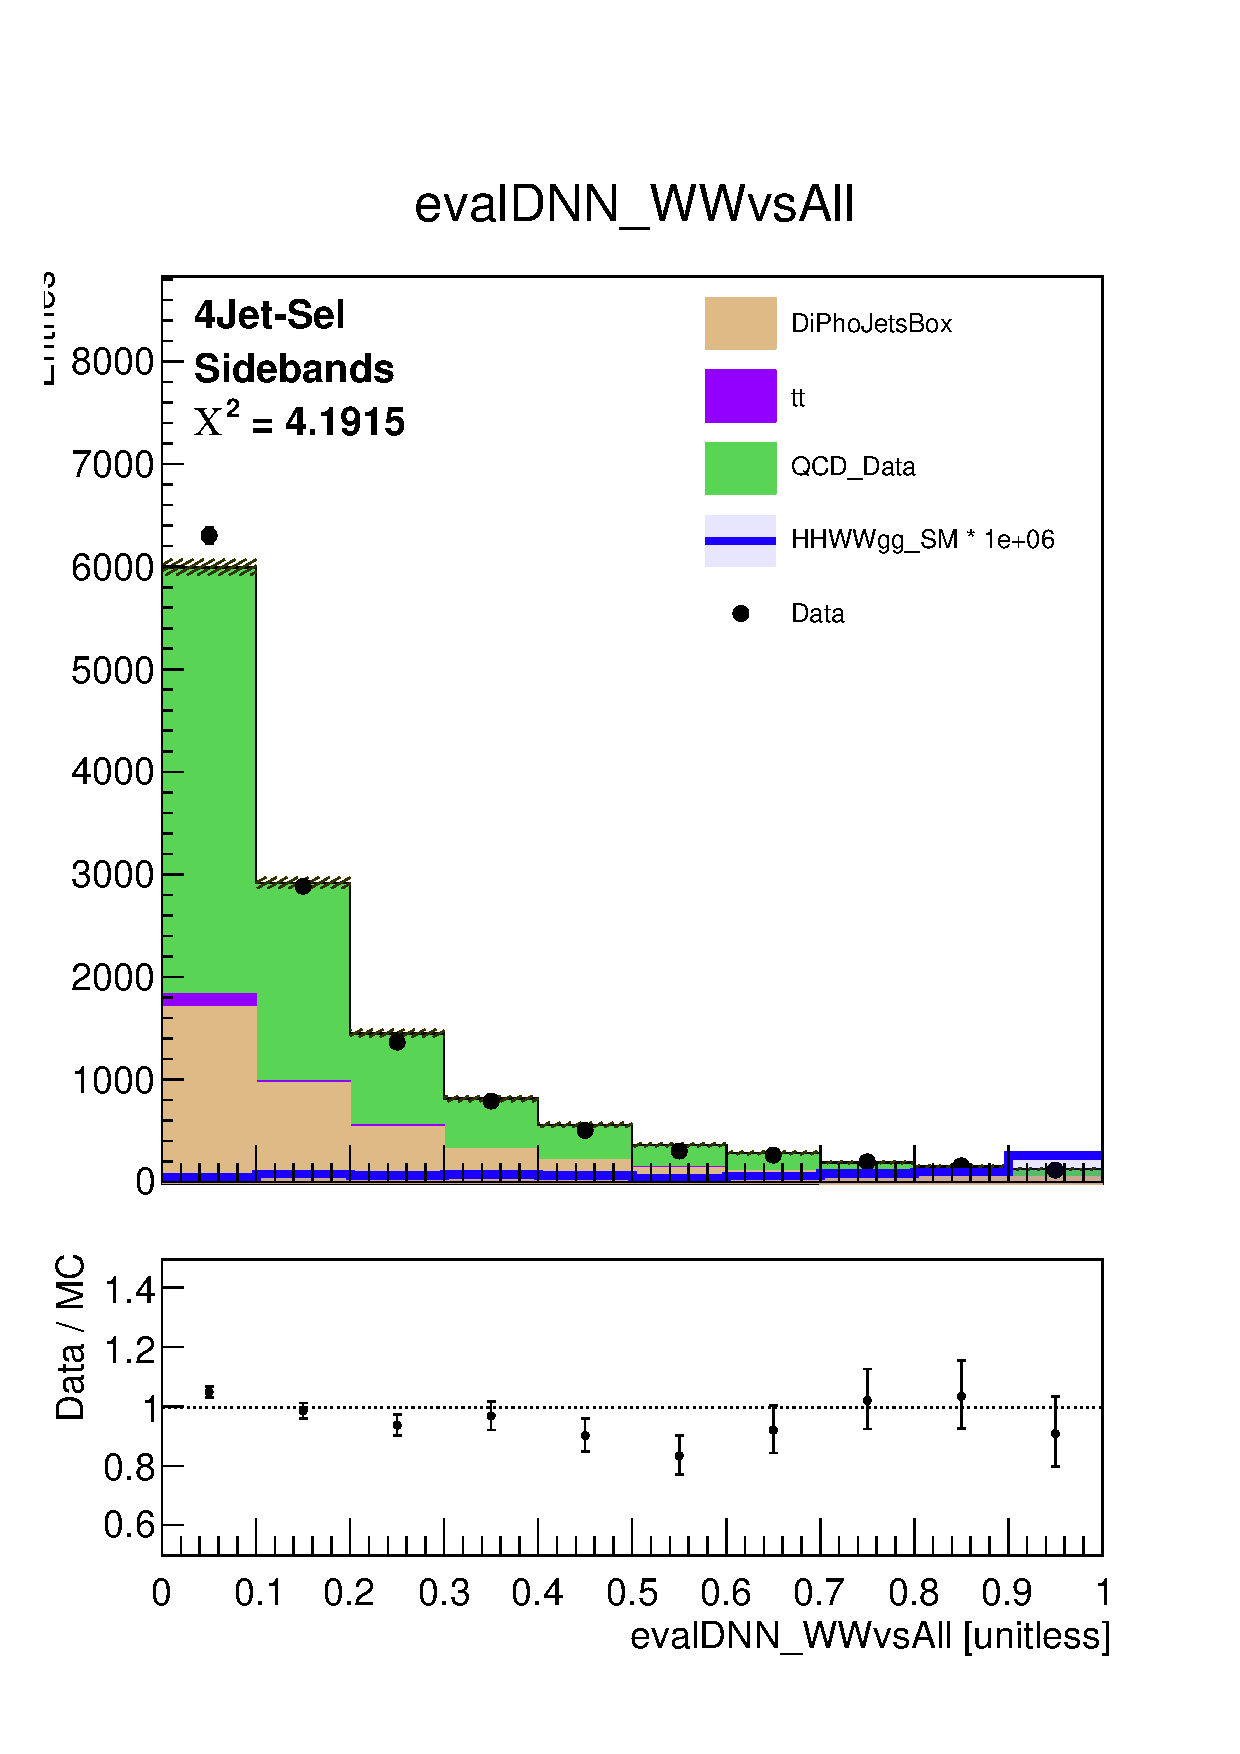
\includegraphics[width=0.45\textwidth]{Images/DataMC/DataMC_evalDNN_WWvsAll_SB_nonLog.pdf}%
  \caption{Data/MC comparison of a fully-hadronic leading DNN input feature and DNN score in the side-band region.}
\label{fig:FH_DataMC_1}
\end{figure}


% \subsection{Semi-leptonic category} \label{sec:SL_Event_Selection}

% Events fall into the SL category if they contain a diphoton candidate and exactly one lepton passing the lepton selections defined in Sec. \ref{sec:Objects}. In this final state, 
a selection is not made on b-tagging score as a preselection, in order to use this as an input feature to the DNN in order to allow it to learn how best to use this score for event discrimination.

% Events used to train the network are required to pass the Semi-Leptonic category selections described in Sec. \ref{sec:event_selection}, which require a diphoton candidate 
% and exactly one lepton passing the common lepton selections described in Sec. \ref{sec:Objects}. 

In the Semi-Leptonic category, in order to separate di-Higgs signal events from the expected single Higgs boson and continuum backgrounds, a multiclass deep neural network is 
trained to identify these three types of processes separately. This optimizes the ability to identify a region of phase space with a maximal number of HH events,
but a minimal number of single Higgs boson and continuum background events. The single Higgs boson processes are markedly different from the continuum background 
processes due to the presence of a diphoton mass peak around 125 GeV originating from the $H\rightarrow\gamma\gamma$ decay. Therefore, 
it is more logical to define these two processes separately in a DNN training rather
than defining them as part of the same class of backgrounds. 

A DNN is trained on a labelled dataset with the di-Higgs process defined as signal, and single Higgs and non-Higgs datasets defined as separate classes. The single Higgs processes
included in the training are the associated VH and ttH$+$Jet production modes of $H\rightarrow\gamma\gamma$.

The samples used for training and labeled as signal are the 12 LO benchmark samples, as well as the LO SM benchmark, where all thirteen use 2017 detector conditions.
When training on these samples, the reweighting procedure described in Sec. \ref{sec:EFT_Description}
is applied to reweight the 13 LO samples to the SM at NLO, in order to increase the statistics used to train the network to identify the SM signal. This leads to a large, statistically independent 
set of events which are reweighted to look like the SM HH signal to be used by the semi-leptonic DNN training. 

% Events used to train the network are required to pass the Semi-Leptonic category selections described in Sec. \ref{sec:event_selection}, which require a diphoton candidate 
% and exactly one lepton passing the common lepton selections described in Sec. \ref{sec:Objects}. 

The single Higgs and continuum backgrounds used in the training are those with a large yield, and with a reasonable absolute number of simulated events after the application of the Semi-Leptonic
category selections. During training, the three processes are defined as separate classes: Namely, events in the signal MC are classified as signal events, events in the single Higgs MC are classified 
as resonant background, and events in the continuum background MC are classified as continuum background. 

Due to the imbalance of the total and weighted number of events between the three datasets, 
a class weight is applied to each class in order to equalize the yields of the three classes. This ensures the network focuses on categorising all three classes with equal importance.

The features used as input to the DNN can be found in Fig. \ref{fig:DNNinputvars}.  Only basic features are used because the network is able
to learn the best way of combining features to provide optimal discrimination between signal and background.
To determine the level of optimization of the network to data, the data-MC ratio is checked for input features in the side-band regions. In order to improve data-MC agreement,
an N-dimensional kinematic reweighting is performed. A per-event weight, called a kinematic weight, is computed using the ratio between background MC and data from the $\mgg$ sideband region. 
The variables leading jet \pt, subleading set \pt, lepton pT, scaled leading photon \pt, scaled subleading photon \pt, and MET are used to calculate this per-event weight. After per events weights
are derived, a fiducial selection is made removing all events which have $|w_{MC}*w_{k}| > 10$, where $w_{MC}$ is the nominal MC weight computed from cross section, luminosity, PU weight,
scale factors and GEN weights, and $w_{k}$ represents the per event kinematic weight. This fiducial selection removes events with very large weights which heavily impact the DNN training in
a non-desirable way.

% \begin{sidewaystable}[!htbp]
% \begin{Figure}[!htbp]
\begin{figure}[!htbp]
  % \topcaption{Input features used to train semi-leptonic and fully-hadronic channel DNNs.}
  \resizebox{\textwidth}{!}{
  \begin{tabular}{| l | l | c | c |}
  \hline
  Feature & Description & Used in SL training & Used in FH trainings \\
  \hline
  Leading Photon p$_T$ / \mgg& \pt of the photon with the highest \pt out of the selected photons, scaled to diphoton mass. & \checkmark & \checkmark \\
  Leading Photon $\eta$ & Pseudorapidity of the photon with the highest \pt out of the selected photons & \checkmark & \checkmark \\
  Leading Photon $\phi$ & Direction in the transverse plane of the photon with the highest \pt out of the selected photons & \checkmark & \checkmark \\
  Leading Photon E / \mgg& Energy of the photon with the highest \pt out of the selected photons, scaled to diphoton mass. & \checkmark &   \\
  Leading Photon MVA & Photon MVA score of the photon with the highest \pt out of the selected photons & \checkmark & \checkmark \\
  Subleading Photon p$_T$  / \mgg& \pt of the photon with the second highest \pt out of the selected photons, scaled to diphoton mass. & \checkmark & \checkmark \\
  Subleading Photon $\eta$ & Pseudorapidity of the photon with the second highest \pt out of the selected photons & \checkmark & \checkmark \\
  Subleading Photon $\phi$ & Direction in the transverse plane of the photon with the second highest \pt out of the selected photons & \checkmark & \checkmark \\
  Subleading Photon E / \mgg & Energy of the photon with the second highest \pt out of the selected photons, scaled to diphoton mass. & \checkmark &   \\
  Subleading Photon MVA & Photon MVA score of the photon with the second highest \pt out of the selected photons & \checkmark & \checkmark \\
  Jet Multiplicity & Number of selected jets in the event (flavor inclusive) & \checkmark & \checkmark \\
  Lepton four-momentum & \pt, pseudorapidity, $\phi$ and energy of the selected lepton & \checkmark & \\
  MET & The missing transverse energy & \checkmark & \checkmark \\
  $M_{T}$(l, MET) & The transverse mass of the selected lepton and MET & \checkmark & \checkmark \\
  $m_{j_{0},j_{1}}$ & The invariant mass of the leading and subleading jets & \checkmark & \checkmark \\

  Leading Jet kinematics and b-score & \pt, pseudorapidity, $\phi$, energy and b-tagging score of the jet with the highest \pt out of the selected jets & \checkmark & \checkmark \\ 
  Subleading Jet kinematics and b-score & \pt, pseudorapidity, $\phi$, energy and b-tagging score of the jet with the second highest \pt out of the selected jets & \checkmark & \checkmark \\ 
  Second Subleading Jet kinematics and b-score & \pt, pseudorapidity, $\phi$, energy and b-tagging score of the jet with the third highest \pt out of the selected jets & & \checkmark \\ 
  Third Subleading Jet kinematics and b-score & \pt, pseudorapidity, $\phi$, energy and b-tagging score of the jet with the fourth highest \pt out of the selected jets & & \checkmark \\ 
  
  $\Delta \phi(HH)$ & Azimuthal separation between the two selection Higgs candidates &   & \checkmark\\
  $\Delta R(HH)$ & Separation between two Higgs in the transverse plane &   & \checkmark\\
  $min(\Delta R(g_k,j_l))$ & minimum separation between the selected jet and photon candidate &   & \checkmark\\
  $max(\Delta R(g_k,j_l))$ & maximum separation between the selected jet and photon candidate &   & \checkmark\\
  $min(\Delta R(j_k,j_l))$ & minimum separation between the jet candidates &   & \checkmark\\
  $max(\Delta R(j_k,j_l))$ & maximum separation between the jet candidates &   & \checkmark\\
  costhetastar & The angle between the parton collision axis $z$ and the $pp\rightarrow H_1H_{2}$ decay axis $z'$, both defined in the $H_1H_{2}$ system rest frame &   & \checkmark \\
  costheta1 & Angle between the direction of the W-boson ($W_1$) from the $H_1\rightarrow W_1 W_2$ and the direction opposite the $H_1H_2$ in the $H_1$ rest frame. &   & \checkmark\\
  costheta2 & Angle between the direction of the W-boson ($W_2$) from the $H_2\rightarrow \gamma \gamma$ and the direction opposite the $H_1H_2$ in the $H_2$ rest frame. &   & \checkmark\\
  Phi & Angle between the decay planes of the two Z-system in the $H_1H_2$ rest frame &   & \checkmark\\
  Phi1 & Angle between the $zz'$ plane and the plane of the $H_{1}\rightarrow \gamma \gamma$ decay in the $H_{1}H_{2}$ rest frame &   & \checkmark \\
  W1 pT & pT of vector sum of two leading jets &   & \checkmark\\
  W1 $\eta$ &  rapidity of vector sum of two leading jets &   & \checkmark\\
  W1 mass &  Invariant mass of vector sum of two leading jets &   & \checkmark\\
  
  W2 pT & pT of vector sum of 3rd and 4th leading jets &   & \checkmark\\
  W2 $\eta$ & rapidity of vector sum of 3rd and 4th leading jets &   & \checkmark\\
  W2 mass & Invariant mass of vector sum of 3rd and 4th leading jets &   & \checkmark\\
  
  WW pT & pT of vector sum of first four leading jets &   & \checkmark\\
  WW $\eta$ & rapidity of vector sum of first four leading jets &   & \checkmark\\
  WW mass & Invariant mass of vector sum of first four leading jets &   & \checkmark\\
  
  \hline
  \end{tabular}
  }
  % \label{tab:DNNinputvars}
\caption{Input features used to train semi-leptonic and fully-hadronic channel DNNs. \label{fig:DNNinputvars}}
\end{figure}
% \end{sidewaystable}

Because the three classes are globally scaled to have matching yields in the training, a single Data/MC weight is extracted and applied in order to compare the data and MC input feature shapes.
The weight is obtained and a shape comparison is performed
in the following way: First, MC is scaled to the ratio of data / MC integrals
in the full mass region, 100 $<$ $\mgg$ $<$ 180 GeV. Then, events with an output DNN discriminant score less than 0.1 are removed before the ratio of data / MC
integrals is computed, to only show the data / MC agreement of events which are used in the Semi-Leptonic categorization and fitting. In this analysis, events with a DNN score less than 0.1 
are removed, and therefore are not used in categorization, nor in any analytic fitting. This is done because this region contains a large portion of background, and a very low portion of signal, and therefore has a negligible impact on the sensitivity of the analysis. Additionally,
this region is not used as a control region to reduce the uncertainty of MC in the signal region.

The MultiClass DNN outputs three DNN scores, each corresponding to the likelihood that an event falls into each of the three classes, which sum to one, and are back-propogated
to optimize the DNN weights. This also means that if an event has a high HH class DNN score, the sum of the H and continuum background DNN scores must be small. As there is no need to separate 
the single Higgs and continuum background processes from each other, only the output HH class DNN score is used in the analysis for categorization.

Several architectures were investigated in an attempt to give the model enough flexibility to model decision boundaries in high-dimensionality
phase-space, while ensuring the model is trainable with the size of our dataset. Once the network's architecture was established, a hyper-parameter scan was performed on the number of epochs, 
learning rate and batch size. The performance of the network was found to be relatively robust to further fine-tuning of hyper-parameters.

The leading importance input features of the network, according to their Shapley values, are the leading and subleading photon $\pt$ taken as a ratio to the invariant diphoton mass, 
the energy of the lepton, and the $\pt$ of the subleading jet. 

The output DNN score comparison between the data and MC for a leading importance variable and the HH DNN score is shown in Figure \ref{fig:SLDNNFeaturecontrolplots-1}. Four categories are defined, with the corresponding DNN score boundaries: 
[0.1, 0.63, 0.84, 0.89, 1.0].

% Note that as the DNN output score is 
% used to categorize events but is not used as a shape in the extraction of any results, any disagreements between data and simulation could lead to a sub-optimal network, but would not lead to any bias in the 
% final results. 

\begin{figure}[!htbp]
  \setcounter{subfigure}{0}
  \centering
  \subfloat[Scaled Leading Photon pt]{\includegraphics[width=0.45\textwidth]{Images/DNN/DataMC/DataMC_Scaled_Leading_Photon_pt_FullRegion_log.pdf}}
  \qquad
  \subfloat[DNN output score]{\includegraphics[width=0.45\textwidth]{Images/DNN/DataMC/DataMC_evalDNN_HH_FullRegion_log.pdf}}
  \caption{Data/MC ratio of semi-leptonic channel leading input feature, and DNN score in diphoton mass region 100 $<$ $\mgg$ $<$ 180 GeV.}
  \label{fig:SLDNNFeaturecontrolplots-1}
\end{figure}

In addition, a separate parametric binary DNN is trained in order to categorize signatures from the twenty EFT benchmark hypotheses defined in Tab. \ref{tab:eft_bench}. A parametric DNN is a
neural network which, in this case, includes the EFT benchmark number as an input variable. This allows one to train a DNN which can effectively produce 20 output scores, based on different 
input values of the node hypothesis, rather than having to train 
20 separate DNN's. This method is particularly useful for training a DNN to categorize events for the 20 EFT benchmark nodes in this analysis. A single DNN training is performed, using 
4 NLO samples reweighted to the 20 EFT benchmarks at NLO as signal, with the same single Higgs and continuum background MC samples used as backgrounds in the training as were used for the DNN 
trained to identify the SM HH signal. Category boundaries are optimized for each node hypothesis scenario, based on expected sensitivity. 


% \subsection{Fully-leptonic category}

% For events to fall into the FL analysis category, they must contain exactly two oppositely charged leptons ($e^{+}e^{-}$, $\mu^{+}\mu^{-}$, $e^{\pm}\mu^{\mp}$).
% The leading \pt lepton is required to have \pt $>$ 20$\GeV$, the subleading lepton is required to have \pt $> 10\GeV$, and a distance parameter between the two leading \pt leptons $>$ 0.4 is required.
% Events are rejected from this category if the event contains a third lepton with \pt $> 10\GeV$ in order to avoid saving events with three high energy leptons, as only two 
% are expected from this process. In order to identify events with missing transverse momentum due to the two neutrinos from the 
% leptonically decaying W-bosons, events are required to have $p_T^{miss} > 20 \GeV$. Furthermore, the diphoton candidate in this final state is required to have \pt $> 91 \GeV$, 
% an invariant mass between each electron candidate and photon candidate which is at least 5 GeV different from the invariant Z boson mass to avoid saving Z$\rightarrow\ell\ell$ events. The invariant mass 
% from the two leading leptons is required to be $<$ 80 GeV or $>$ 100 GeV in order to suppress VH(H$\rightarrow\gamma\gamma$) events, as shown in Fig.\ref{fig:FL_dilepmass}. In addition, events containing at least one jet 
% with a b-tagging score greater than a medium working point are removed. The reason a b-veto is applied in this final state and not for the SL and FH final states is because this final state applies 
% a cut-based selection, and therefore we choose to apply a b-veto as part of the final selections. 

% \begin{figure}[!htbp]
%   \begin{center}
% 	\includegraphics[width=0.9\textwidth]{Images/Selections/FL_CutBased/DiLeptonMass.pdf}
%     \caption{
%       $m_{ll}$ distribution comparison between signal and VH events, where the signal and VH distributions have been normalized to 1, and the two dashed lines show the final cuts on the di-Lepton mass: $m_{ll}$ $< 80\GeV$ or $m_{ll}$ $> 100\GeV$ .
%     }
%     \label{fig:FL_dilepmass}
%   \end{center}
% \end{figure}

